\documentclass[logo,reportComp]{thesis}
\usepackage[cpp,linenum]{mypackage}

\title{计算机网络实验报告}
\subtitle{实验一:数据表示实验}
\school{数据科学与计算机学院}
\author{陈鸿峥}
\classname{17大数据与人工智能}
\stunum{17341015}
\headercontext{计算机网络实验报告}

\begin{document}

\maketitle

\section{实验目的}
掌握结构数据的保存和读取方法。

\section{实验说明}
\begin{itemize}
	\item 把源程序和可执行文件放在相应的上交源码目录中
	\item 截屏用按键(Ctrl+Alt+PrintScreen)截取当前窗口
	\item 把每段具有独立功能的代码单独写入一个函数有助于编码和调试
\end{itemize}

\section{参考资料}
\begin{itemize}
	\item C语言字符串函数:{\small\url{http://msdn.microsoft.com/zh-cn/library/f0151s4x(v=vs.110).aspx}}
	\item C++文件流:{\small\url{http://www.cplusplus.com/doc/tutorial/files/}}
\end{itemize}

\section{实验环境}
本机为Windows 10 + gcc 7.3.0

\section{实验内容}
\subsection{结构数据保存和读出(StructSave.cpp)}
\subsubsection{实验要求}
循环输入员工(\verb'Person')的信息,每输入一个员工的信息,立即写入文件(\verb'Persons.stru'),直到输入的姓名为\verb'exit'时跳出循环。
然后读出该文件,显示每个\verb'Person'的信息。

\verb'Person'的信息表示:
\begin{lstlisting}
struct Person {
   char username[USER_NAME_LEN];
   int level;
   char email[EMAIL_LEN];
   DWORD sendtime;
   time_t regtime;
}; 
\end{lstlisting}

\subsubsection{运行结果}
控制行运行结果如下,并在当前文件夹中产生文件\verb'Persons.stru'。
注意这里将用户输入和程序输出分开为两个部分。
\begin{figure}[H]
\centering
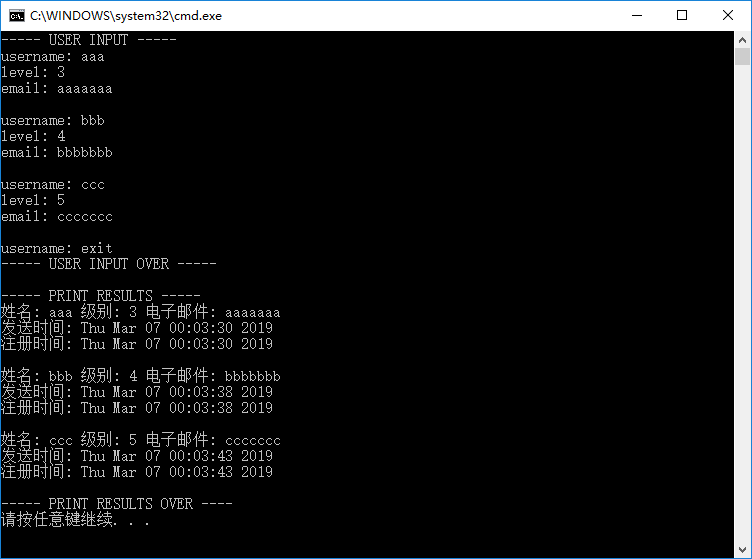
\includegraphics[width=0.8\linewidth]{fig/StructSave.PNG}
\end{figure}

\subsubsection{源代码}
\begin{lstlisting}
#include <stdio.h>
#include <stdlib.h>
#include <string.h>
#include <time.h>

#define BUF_LEN 100
#define USER_NAME_LEN 20
#define EMAIL_LEN 80
#define TIME_BUF_LEN 30
#define MAX_INT 0x3f3f3f3f

typedef unsigned long DWORD;

typedef struct Person {
    char username[USER_NAME_LEN];
    int level;
    char email[EMAIL_LEN];
    DWORD sendtime;
    time_t regtime;
} Person;

int inputOnePerson(FILE* pfile)
{
	Person person;
	
	fflush(stdin);
	char name[USER_NAME_LEN];
	printf("username: ");
	gets(name);
	if (strcmp(name,"exit") == 0)
		return 0;
	strcpy(person.username,name);
	fprintf(pfile, "%s\n", name);

	int l;
	printf("level: ");
	scanf("%d",&l);
	person.level = l;
	fprintf(pfile, "%d\n", l);

	char email[EMAIL_LEN];
	printf("email: ");
	scanf("%s",&email);
	strcpy(person.email,email);
	fprintf(pfile, "%s\n", email);

	time_t now; // current time
	time (&now);  // get now time
	struct tm* lt = localtime (&now);
	person.sendtime = (DWORD)now;
	person.regtime = now;
	fprintf(pfile, "%ld\n", person.sendtime);
	fprintf(pfile, "%ld\n", person.regtime);

	printf("\n");
	return 1;
}

int main()
{
	FILE* pfile;
	int i;
	// Input
	pfile = fopen("./Persons.stru","wb");
	printf("----- USER INPUT -----\n");
	for (i = 0; i < MAX_INT; ++i)
		if (!inputOnePerson(pfile))
			break;
	fclose(pfile);
	printf("----- USER INPUT OVER -----\n\n");

	// Read the file
	pfile = fopen("Persons.stru","r");
	if (pfile == NULL)
		exit(EXIT_FAILURE);
	printf("----- PRINT RESULTS -----\n");
	for (i = 0; i < MAX_INT; ++i){
		char name[USER_NAME_LEN];
		if (fscanf(pfile,"%s",name) != 1)
			break;
		printf("`姓名': %s ", name);

		int l;
		fscanf(pfile,"%d",&l);
		printf("`级别': %d ", l);

		char email[EMAIL_LEN];
		fscanf(pfile,"%s",email);
		printf("`电子邮件': %s\n",email);

		char buf[TIME_BUF_LEN];
		time_t sendtime;
		fscanf(pfile,"%ld",&sendtime);
		struct tm* lt = localtime (&sendtime);
		// Www Mmm dd hh:mm:ss yyyy\n
		strftime(buf,TIME_BUF_LEN,"%a %b %d %H:%m:%S %Y",lt);
		printf("`发送时间': %s\n", buf);
		
		time_t regtime;
		fscanf(pfile,"%ld",&regtime);
		lt = localtime (&regtime);
		strftime(buf,TIME_BUF_LEN,"%a %b %d %H:%m:%S %Y",lt);
		printf("`注册时间': %s\n", buf);

		printf("\n");
	}
	printf("----- PRINT RESULTS OVER ----\n");
	fclose(pfile);
	return 0;
}
\end{lstlisting}

\subsection{多文件合并保存和读出(FilePack.cpp)}
\subsubsection{实验要求}
循环输入多个文件名(不超过200MB,可以自己确定),每输入一个,就把该文件的文件名(最多300字节)、文件大小(long)和文件内容写入文件\verb'FileSet.pak'中,输入文件名为\verb'exit'时跳出循环。
然后读\verb'FileSet.pak',每读出一个文件就把它保存起来,有重名文件存在时文件名加上序号(从2开始)。

注意:合并时可以先取得文件大小,然后边读边写。

\subsubsection{运行结果}
\verb'E:\Test'下的三个文件:\verb'Convex_Optimization.pdf'、\verb'test.PNG'、\verb'TeXbyTopic.pdf',并有一个空文件夹\verb'E:\Test\TestOut'
\begin{figure}[H]
\centering
\begin{tabular}{c}
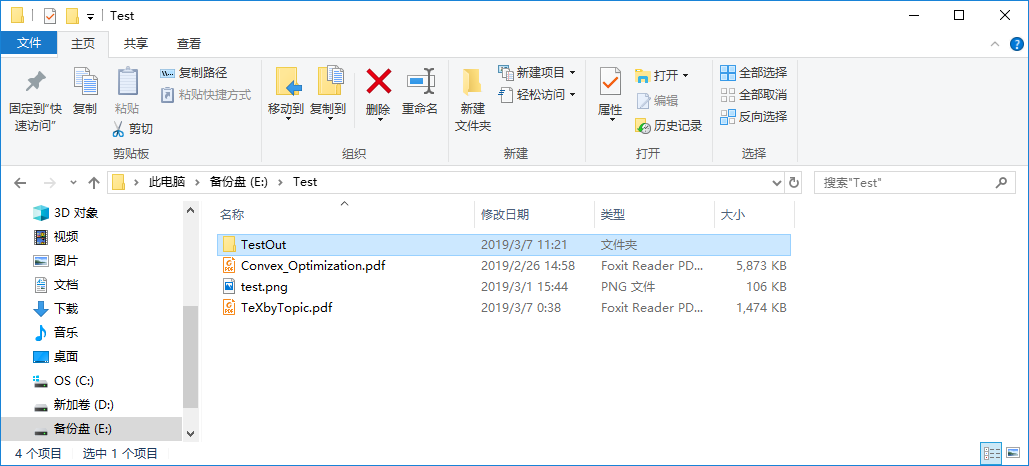
\includegraphics[width=0.8\linewidth]{fig/FilePack-1.PNG}\\
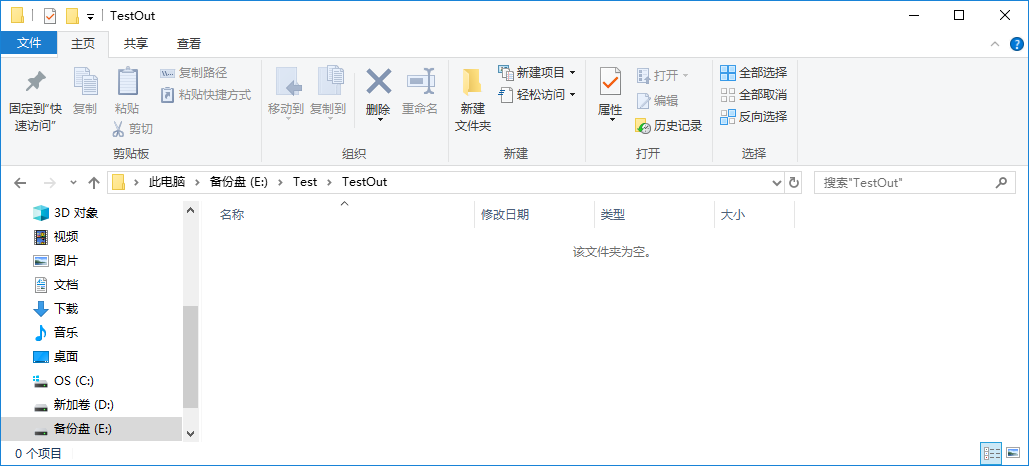
\includegraphics[width=0.8\linewidth]{fig/FilePack-2.PNG}
\end{tabular}
\end{figure}

运行程序控制行结果如下
\begin{figure}[H]
\centering
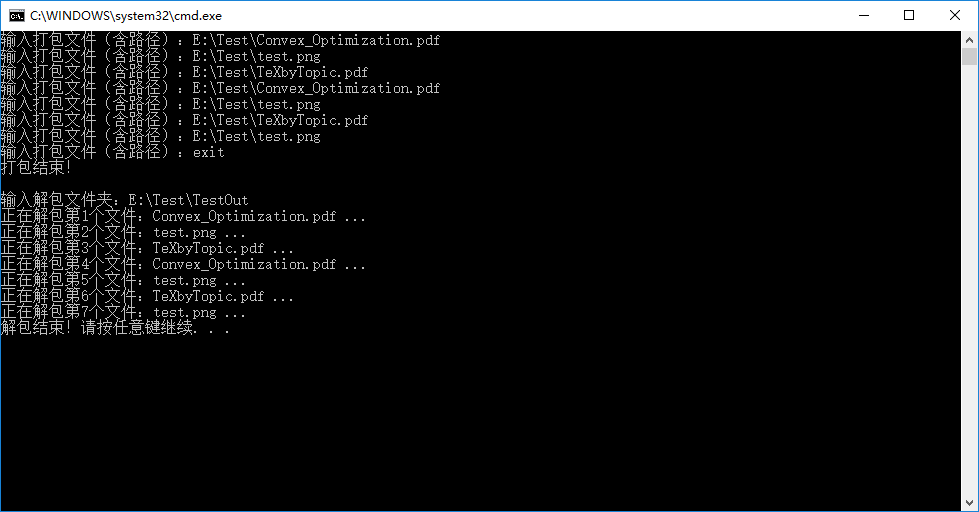
\includegraphics[width=0.8\linewidth]{fig/FilePack-3.PNG}
\end{figure}

注意在我的程序中\verb'FileSet.pak'生成位置与执行文件\verb'FilePack.exe'的位置相同,在这里没有显示出来,但文件大小与所有打包文件大小之和相同。

文件生成展示如下,见最后一列可见生成文件与原文件大小相同。
\begin{figure}[H]
\centering
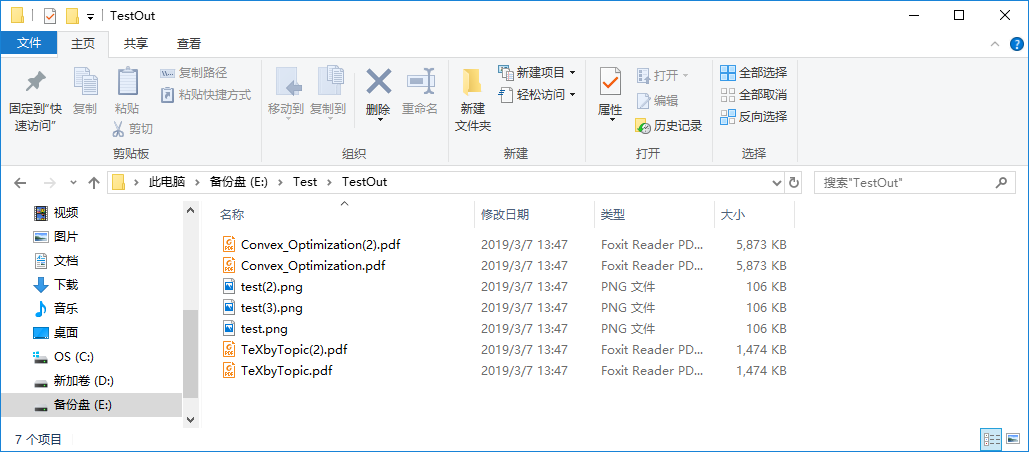
\includegraphics[width=0.8\linewidth]{fig/FilePack-4.PNG}
\end{figure}

\subsubsection{与同学互测并截屏运行结果}
把保存的文件(\verb'FileSet.pak')给同学,看他是否可以可以取出其中文件,同样可以测试是否可以读出并保存同学的文件。
注意结构要相同。

\textbf{为方便测评,在我的程序中添加了从命令行读入指令的操作(源程序121行),如果读入指令为1,则直接进行解压操作。}

原来的文件夹\verb'E:\CrossTest'中只有执行文件和\verb'pak'文件。
\begin{figure}[H]
\centering
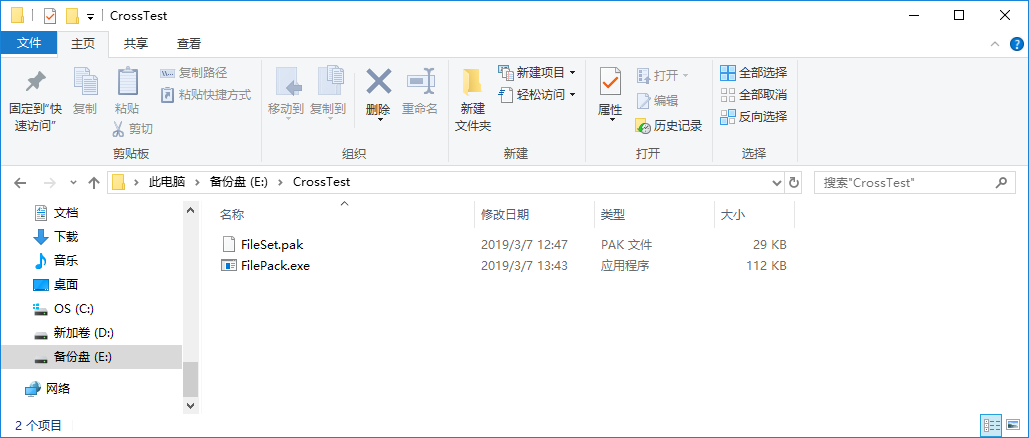
\includegraphics[width=0.8\linewidth]{fig/CrossTest-1.PNG}
\end{figure}

命令行执行
\begin{figure}[H]
\centering
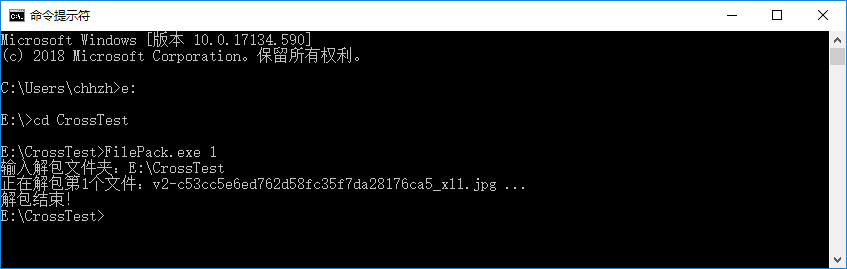
\includegraphics[width=0.8\linewidth]{fig/CrossTest-2.PNG}
\end{figure}

从下面的结果可以看出我的程序可以成功解压同学的\verb'FileSet.pak'文件,并生成对应图片且可以正常打开。
\begin{figure}[H]
\centering
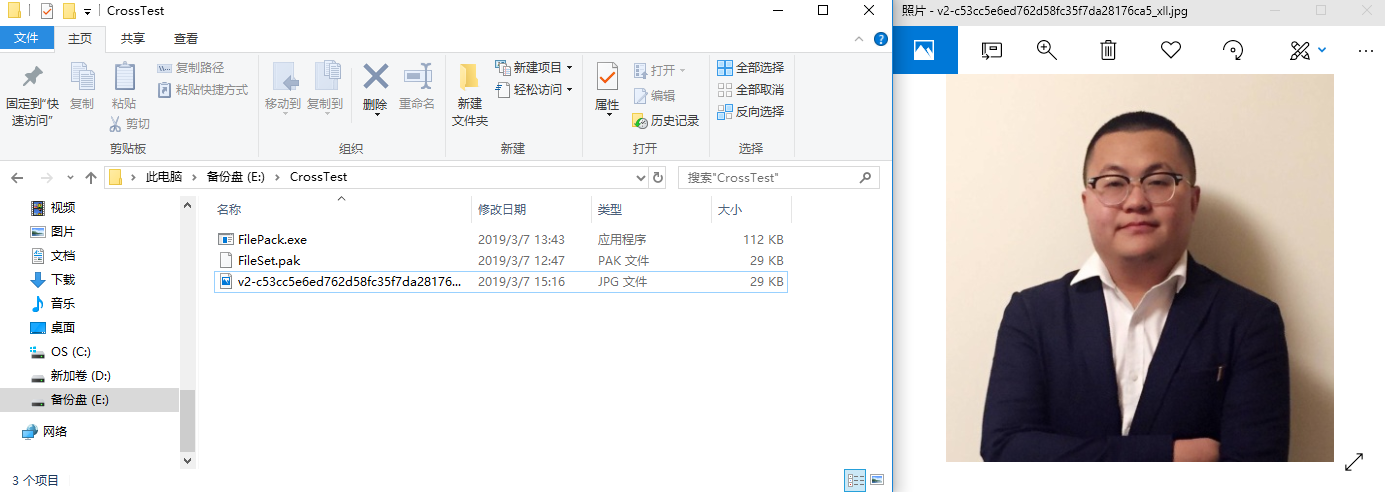
\includegraphics[width=0.8\linewidth]{fig/CrossTest-3.PNG}
\end{figure}

\subsubsection{源代码}
\begin{lstlisting}
#include <iostream>
#include <fstream>
#include <cstdlib>
#include <unistd.h>
#include <string>
using namespace std;

#define PAK_FILE_PATH "FileSet.pak"

class FileClass
{
public:
	FileClass(const string _filepath):
		filepath(_filepath){};

	string getFileName()
	{
		if (filename != "")
			return filename;
		for (int i = filepath.size() - 1; i >= 0; --i)
			if (filepath[i] != '\\')
				filename = filepath[i] + filename;
			else
				break;
		return filename;
	}

	ifstream::pos_type getSize()
	{
	    ifstream in(filepath, ifstream::ate | ifstream::binary); // at the end of file
	    return in.tellg();
	}

	ifstream getStream()
	{
		ifstream input(filepath, ios::binary);
		return input;
	}

private:
	string filepath;
	string filename;
};

bool packFile(const string src, const string dst)
{
	FileClass infile(src);
	ofstream outfile(dst, ios::app|ios::binary); // append

	outfile << infile.getFileName() << endl;
	outfile << infile.getSize() << endl;
	ifstream input = infile.getStream();
	string str;
	while (getline(input,str))
		outfile << str << endl;

	outfile.close();
	return true;
}

bool unpackFile(const string srcFile, const string dstPath)
{
	ifstream input(srcFile,ios::binary);
	string dst = dstPath;
	for (int i = 1; true ; ++i){
		string str, filename;
		if (!getline(input,filename))
			break;
		if (filename == "")
			if (!getline(input,filename))
				break;
		if (filename.find("/") != -1 || filename.find("\\") != -1)
			for (int i = filename.length() -1; i >= 0; --i)
				if (filename[i] == '/' || filename[i] == '\\'){
					filename = filename.substr(i+1,filename.length()-i);
					break;
				}
		cout << "`正在解包第'" << i << "`个文件:'" << filename << " ..." << endl;
		getline(input,str); // size
		streampos size = stol(str);

		// cout << "FileName: " << filename << endl;
		// cout << "Size: " << exp_size << endl;

		fstream output_file;
		// get output file name
		string path;
		if (dst[dst.length()-1] != '\\')
			dst += "\\";
		int cnt = 1;
		while (true){
			if (cnt == 1)
				path = dst + filename;
			else{
				int index = filename.find(".");
				if (index != -1){
					string suffix = filename.substr(index,filename.size()-index);
					path = dst + filename.substr(0,index)
						 + "(" + to_string(cnt) + ")" + suffix;
				} else {
					path = dst + filename + "(" + to_string(cnt) + ")";
				}
			}
			if (access(path.c_str(), F_OK) == -1) // should NOT use fstream
				break;
			cnt++;
		}

		ofstream output(path, ios::out|ios::binary);
		char* memblock = new char [size];
		input.read(memblock,size);
		output.write(memblock,size);
		output.close();

		delete [] memblock;
	}
}

int main(int argc, char *argv[])
{
	if (argc == 1){
	ofstream output(PAK_FILE_PATH); // initialization
	output.close();
	while (true){
		cout << "`输入打包文件(含路径):'";
		string src_file_path;
		getline(cin,src_file_path);
		if (src_file_path == "exit")
			break;

		packFile(src_file_path,PAK_FILE_PATH);
	}
	cout << "`打包结束!'\n" << endl;
	}

	cout << "`输入解包文件夹:'";
	string output_path;
	cin >> output_path;
	
	unpackFile(PAK_FILE_PATH,output_path);

	cout << "`解包结束!'";
	return 0;
}
\end{lstlisting}

\section{完成情况}
\begin{itemize}
	\item 是否完成以下步骤?(\cmark 完成\quad\xmark 未做)\\
	1. [\cmark]\qquad 2. [\cmark]
	\item 是否与同学进行了互测? [\cmark] \\
	互评同学学号姓名:17341059黄杨峻
\end{itemize}

\section{实验体会}
% 写出实验过程中遇到的问题,解决方法和自己的思考;并简述实验体会(如果有的话)。
虽然该实验比较简单,但还是遇到了比较多的问题。

因为平常经常写C++程序,C的文件流操作很多都已经忘了,因而\textbf{第一个实验}对于\textbf{字符串的操作处理}并不得心应手。
查了很多C的字符串函数,才顺利完成任务。
特别要注意判断空行和判断文件末(EOF)的方法。

同时如果要输出中文字符,\verb'cpp'文件注意要保存成GBK编码,否则保存为UTF-8都无法正常输出中文。

对于\textbf{第二个实验},最大的难点则是判断每一个文件到\textbf{哪里终止},因为在\verb'FileSet.pak'中,所有文件都存储在一起,又没有行号标识就很难分开。

因而要通过文件大小来判断。
一开始的方法是每写入一行就获取一次文件大小,但这样子的速度非常非常慢,解码5M的文件竟然用了五分多钟。
后来采用C的buffer方法(见程序111行),解码几十M的文件都能在1秒内完成。

还有要注意文件的命名,需要判重,如果出现重名文件,加序号区分。
这一部分不复杂,但也消耗了几十行的代码(见程序91$\thicksim$107行)。

同样,对于C++二进制文件\verb'ios::binary'的读写操作也查了很多资料才明白其中原理。

最后一点则是要考虑各种极端情况,增强程序的鲁棒性,这样才能适应各种问题。
比如在互测过程中,同学保存的文件名还包括了文件路径,而我的原始程序中并没有处理这一点,因而需要进行预处理后(程序72$\thicksim$77行)才能正常运行。

总的来说,第一次计网实验自己实现了文件单机传输任务,重新熟悉了C语言的使用,学到了很多东西。

\end{document}
% 【交实验报告】
% 每位同学单独完成本实验内容并填写实验报告。
%     交作业地点:http://172.18.187.9/netdisk/default.aspx?vm=17net 
% 编程实验 
% 截止日期:2019年3月9日23:00(周六)。
% 上传文件:学号_姓名_数据表示实验报告.doc
% 学号_姓名_数据表示实验源码.rar (源程序和可执行程序)